This section describes the implications of an existing parallel application that uses one of the supported interfaces such as NetCDF4/HDF5.
The semantics of the API calls will change slightly but typically in a way that is backwards compatible.

\subsection{Logical View}


\begin{figure}
	\centering
	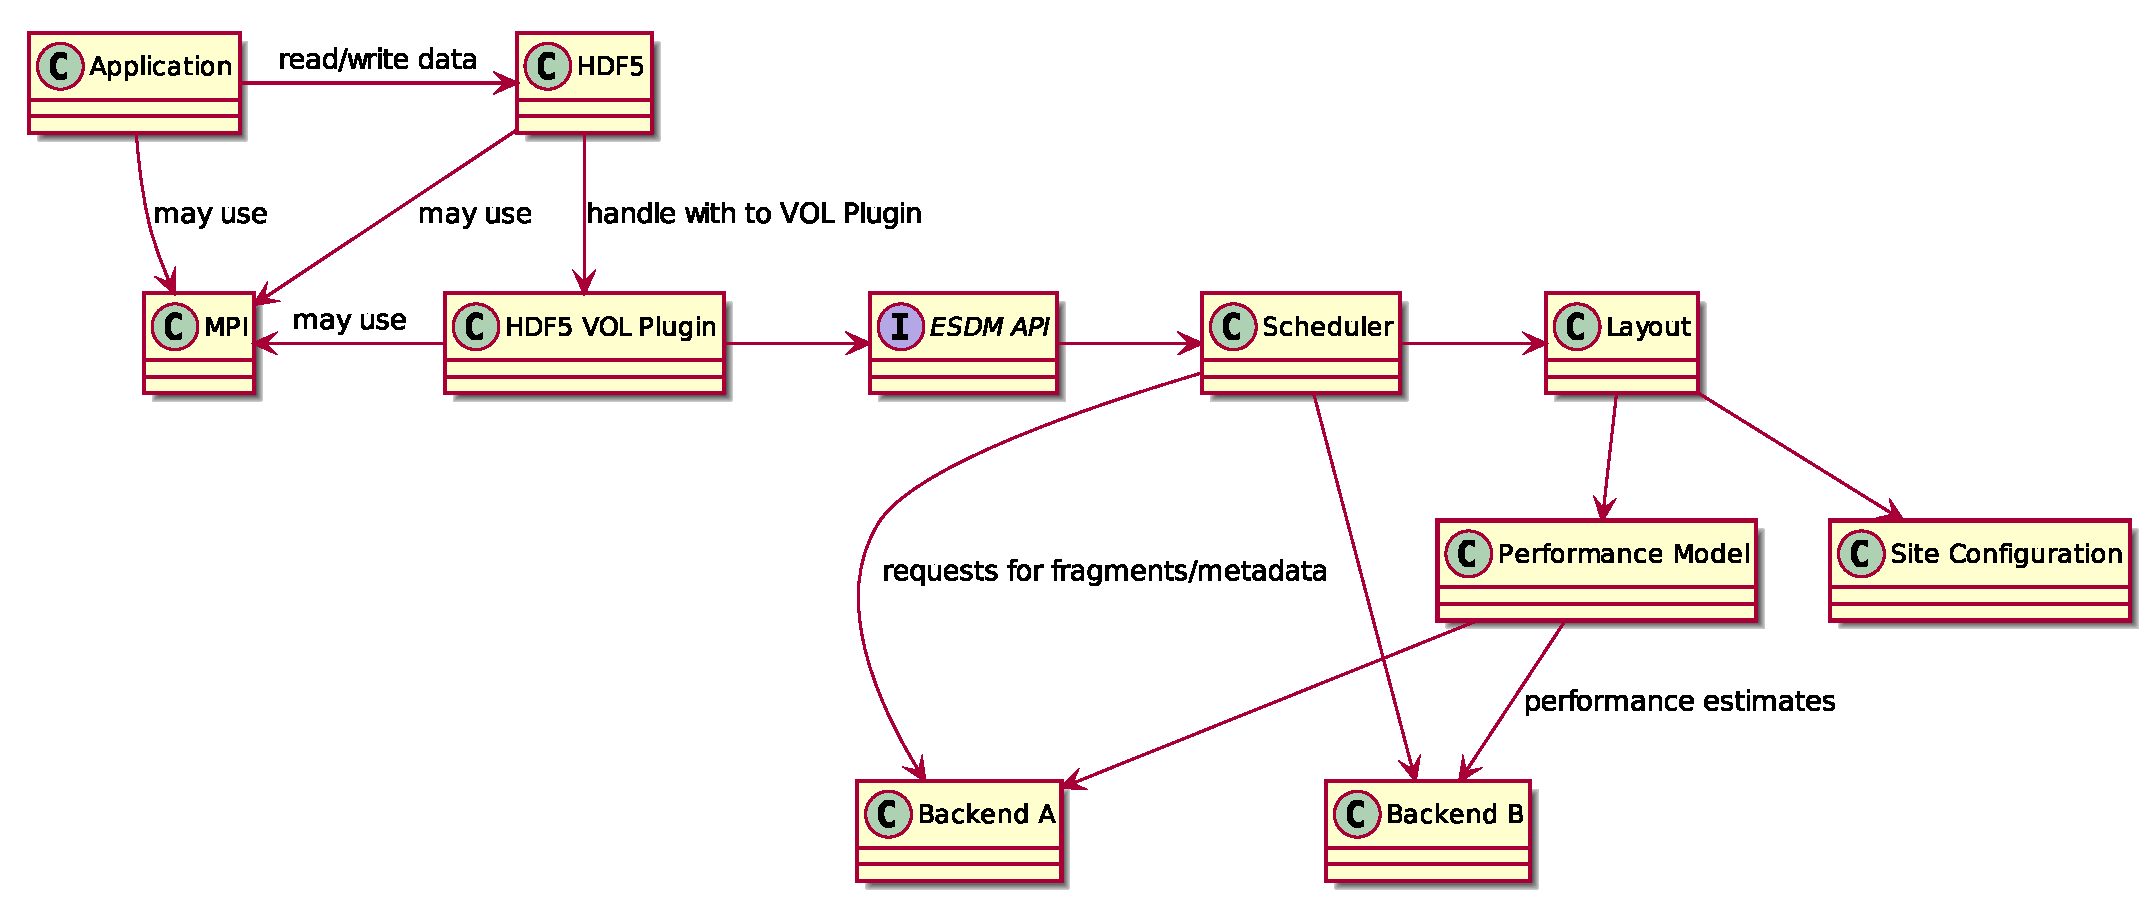
\includegraphics[width=\linewidth]{esdm-hdf5+mpi/logical.eps}
	\caption{Logical view to the HDF+MPI plugin.}
	\label{fig:esdm hdf5 logical view}
\end{figure}

This subsection covers dealing with filenames, opening and closing of containers as well as concurrency semantics.
We assume an MPI parallelised application uses HDF5 with MPI support, e.g., parallel HDF5.
The component diagram in \Cref{fig:esdm hdf5 logical view} illustrates how an HDF5/NetCDF ESDM frontend would mediate between the ESDM and an application.
In addition, multiple processes using ESDM can coordinate using MPI, though only the ESDM component using MPI is the ESDM HDF5 VOL Plugin.




\subsubsection{Dealing with file names}

Traditionally, when opening a file with NetCDF, the filename specifies the location, i.e., a URI where the data resides on a storage system.
We change the notion of the file name to be the descriptor for a virtual container (virtual container descriptor).
The virtual container can be composed of multiple URIs to integrate different variables into one virtual environment on the fly.
Thus, from the reader's perspective, it does not matter if data of a model is split into one or multiple physical files; upon read, all those files can be loaded together as if they would already exist in one logical file.
It is also possible to avoid the use of the metadata backend; by specifying the locations of the variables on existing storage media, they can be linked into a virtual container.
One restriction to this approach is the limitation of the length of file names.
To avoid this limitation, we support a prefix to the filename: \texttt{esd-cfg:/} that leads to a simple JSON file that contains the actual definition of the container.

\subsubsection{Open}

Opening a container (as defined by the file name) in ESDM will trigger the master process within the communicator to retrieve the necessary metadata from ESDM and broadcast it to all participating processes.
Since the metadata is serialisable to JSON, we can exchange the metadata easily.

\subsubsection{Concurrency semantics}

In general, the system is designed for parallel applications of which processes access data independently of each other.
Still, metadata of internal objects such as containers and variables should be managed and updated explicitly by a single process of the application.
That means, within one parallel (MPI) application, some coordination must take place to allow the shared access to containers, variables and shards.
Correct implementation for this behaviour will be performed within the HDF5 VOL plugin.

Data sharing between independent applications is intended to happen after an epoch has been completed.
It is not allowed that multiple parallel applications write data to the same variable at the same time which is considered to be sufficient for most scenarios. A model produces some output and once the epoch is completed the generated data is post-processed.

\subsubsection{Close}

From the user perspective, closing a file that was opened in write mode, will make the content of the file visible in ESDM and durable for subsequent accesses.
Thus, it updates the metadata, for example, incrementing the epoch of the variables and containers modified and updating the reference counters.

\subsection{Physical View}


\begin{figure}
	\centering
	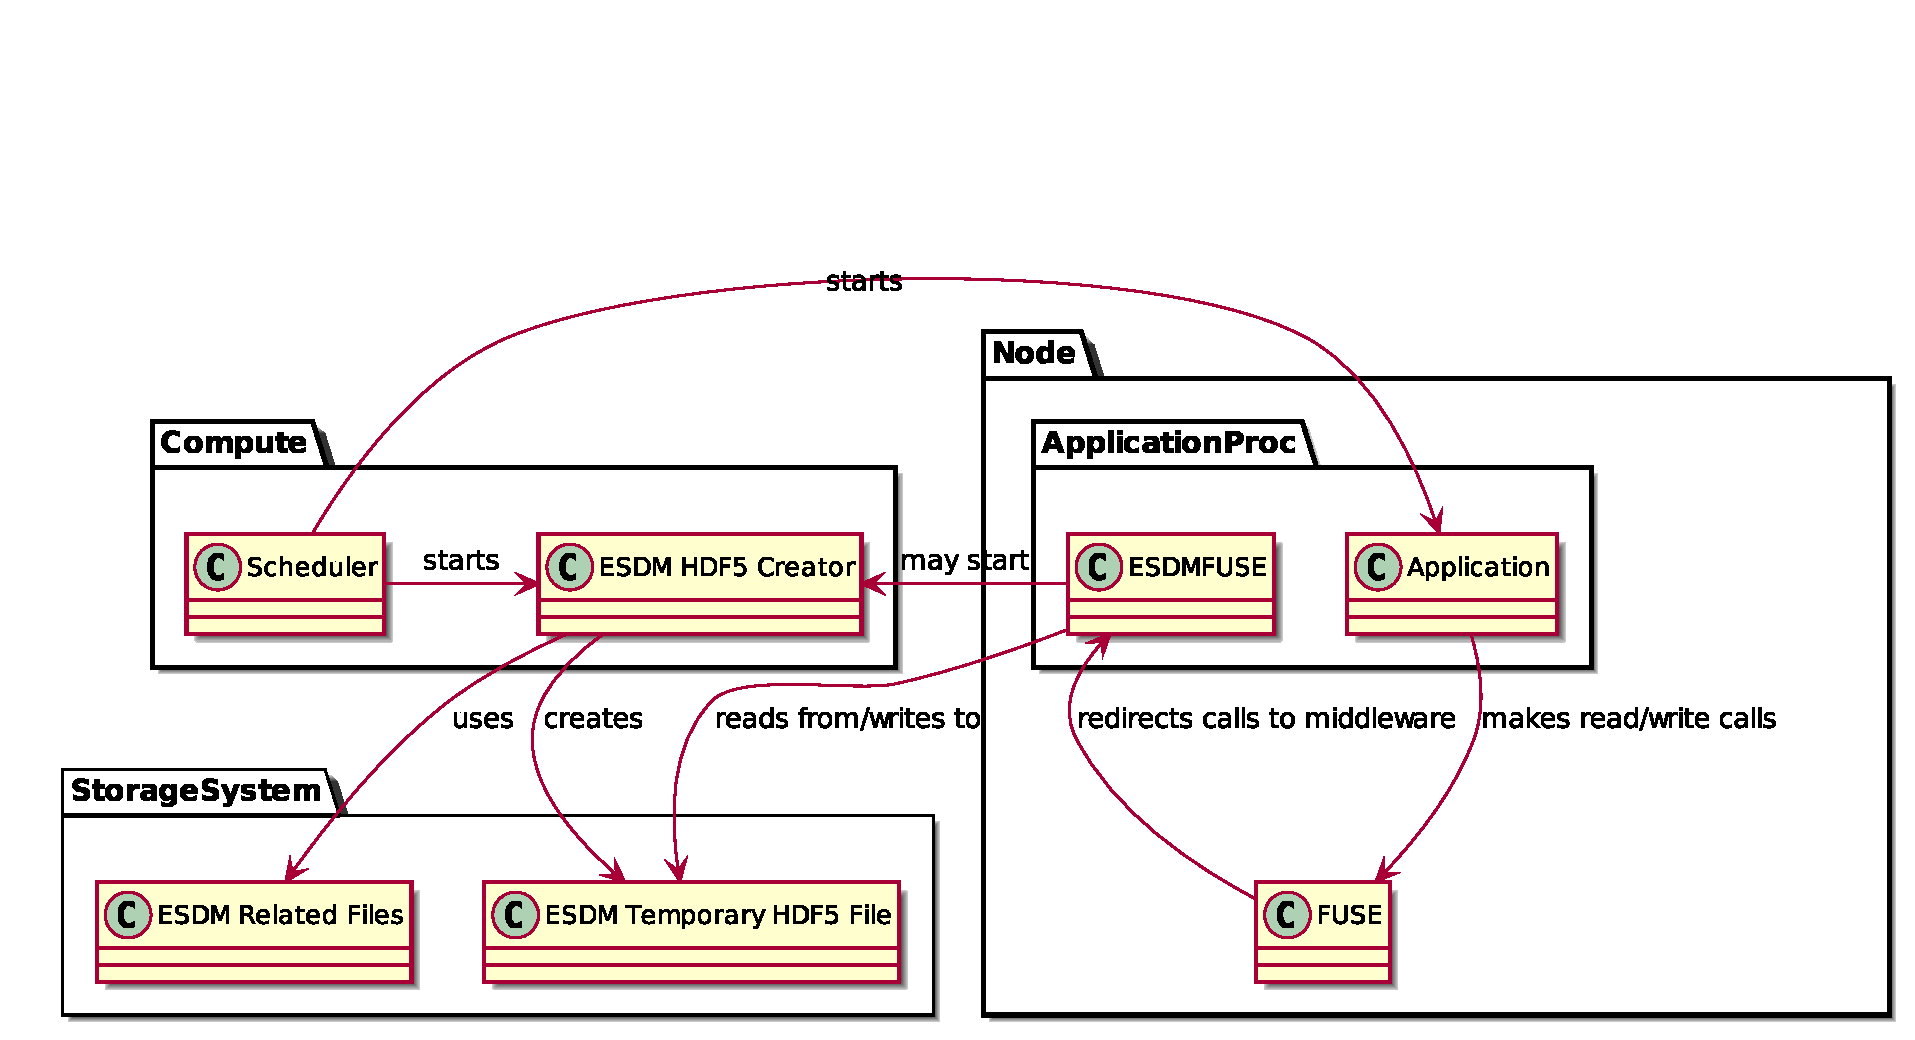
\includegraphics[width=\linewidth]{esdm-hdf5+mpi/physical.eps}
	\caption{Physical view to the HDF5+MPI plugin.}
	\label{fig:esdm hdf5 physical view}
\end{figure}

ESDM does not change anything of the placement of the processes run by MPI.
\Cref{fig:esdm hdf5 physical view} illustrates the distribution and relation of the components across different hardware components.


\subsection{Process View}

\begin{figure}
	\centering
	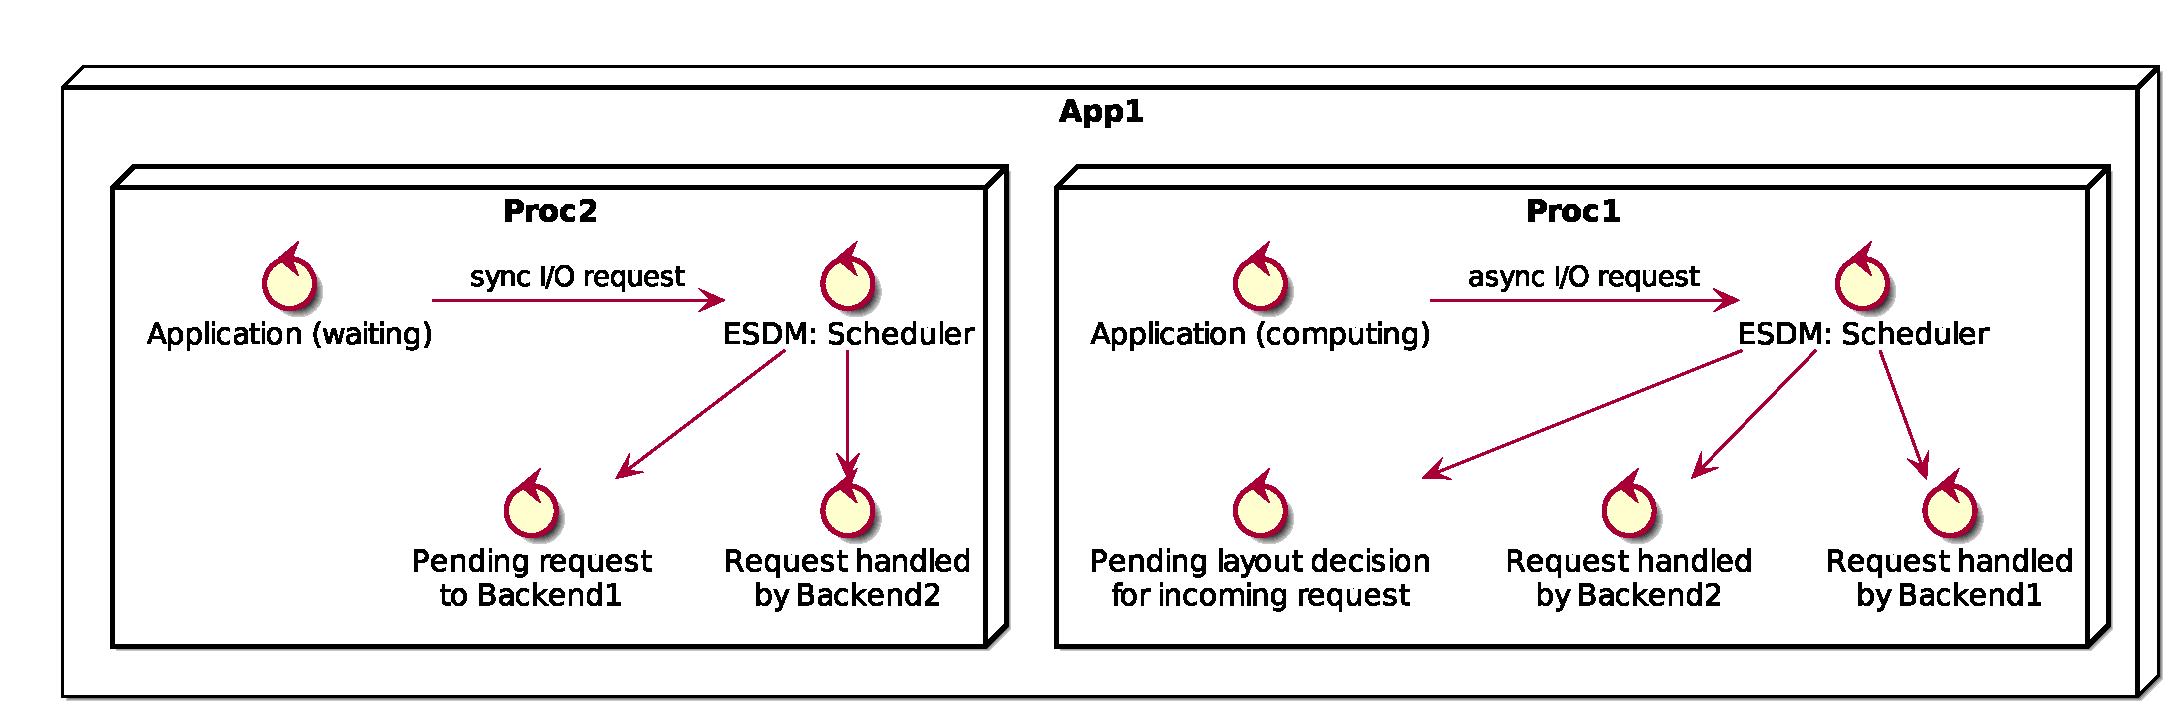
\includegraphics[width=\linewidth]{esdm-hdf5+mpi/process.eps}
	\caption{Process view to the HDF5+MPI plugin.}
	\label{fig:esdm hdf5 process view}
\end{figure}

ESDM will start threads internally in the Scheduler component. However, these threads will not call MPI functions or HDF5.
The ESDM plugin in the HDF5 VOL may use MPI functions (or the lightweight library) to coordinate access to central data structures.
\Cref{fig:esdm hdf5 process view} illustrates the process view as far as the HDF5 VOL plugin and MPI coordination are concerned.
